% !TeX encoding = UTF-8

%% ------------------------------------------------------------------------
%% Copyright (C) 2021 SJTUG
%% 
%% SJTUBeamer Example Document by SJTUG
%% 
%% SJTUBeamer Example Document is licensed under a
%% Creative Commons Attribution-NonCommercial-ShareAlike 4.0 International License.
%% 
%% You should have received a copy of the license along with this
%% work. If not, see <http://creativecommons.org/licenses/by-nc-sa/4.0/>.
%% -----------------------------------------------------------------------

\documentclass[xcolor=table,dvipsnames,svgnames,aspectratio=169]{ctexbeamer}
% 可以通过 fontset=macnew / fontset=ubuntu / fontset=windows 选项切换字体集

\usepackage{tikz}
\usepackage[normalem]{ulem}
\usetikzlibrary{arrows}
\usepackage{amsmath}
\usepackage{mflogo}
\usepackage{graphicx}
\usepackage{xspace}
\usepackage{amsmath}
\usepackage{unicode-math}
\usepackage{ccicons}
\usepackage{hologo}
\usepackage{colortbl}
\usepackage{shapepar}
\usepackage{hyperxmp}
\usepackage{booktabs}
\usepackage{qrcode}
\usepackage{listings}
\usepackage{tipa}
\usepackage{multicol}
\usepackage{datetime2}
\usepackage{fontawesome5}
\usepackage{hyperref}
\usepackage[backend=biber,style=gb7714-2015]{biblatex}

\addbibresource{thesis.bib}
\setbeamertemplate{bibliography item}[text]

\graphicspath{{figures/}}

\hypersetup{
  pdfsubject = {上海交通大学图书馆专题培训讲座},
  pdfauthor = {Alexara Wu},
  pdfcopyright = {Licensed under CC-BY-SA 4.0. Some rights reserved.},
  pdflicenseurl = {http://creativecommons.org/licenses/by-sa/4.0/},
  unicode            = true,
  psdextra           = true,
  pdfdisplaydoctitle = true
}

\pdfstringdefDisableCommands{
  \let\\\relax
  \let\quad\relax
  \let\hspace\@gobble
}

\renewcommand{\TeX}{\hologo{TeX}}
\renewcommand{\LaTeX}{\hologo{LaTeX}}
\newcommand{\BibTeX}{\hologo{BibTeX}}
\newcommand{\XeTeX}{\hologo{XeTeX}}
\newcommand{\pdfTeX}{\hologo{pdfTeX}}
\newcommand{\LuaTeX}{\hologo{LuaTeX}}
\renewcommand{\CTeX}{C\TeX}
\newcommand{\MiKTeX}{\hologo{MiKTeX}}
\newcommand{\MacTeX}{Mac\hologo{TeX}}
\newcommand{\beamer}{\textsc{beamer}}
\newcommand{\XeLaTeX}{\hologo{Xe}\kern-.13em\LaTeX{}}
\newcommand{\pdfLaTeX}{pdf\LaTeX{}}
\newcommand{\LuaLaTeX}{Lua\LaTeX{}}

\def\TeXLive{\TeX{} Live\xspace}
\let\TL=\TeXLive
\newcommand{\SJTUThesis}{\textsc{SJTUThesis}\xspace}
\newcommand{\SJTUBeamer}{\textsc{SJTUBeamer}\xspace}
\newcommand{\SJTUThesisVersion}{1.0.0rc7}
\newcommand{\SJTUThesisDate}{2020/7/31}

\newcommand\link[1]{\href{#1}{\faLink}}
\newcommand\pkg[1]{\texttt{#1}}

\def\cmd#1{\texttt{\color{DarkBlue}\footnotesize $\backslash$#1}}
\def\env#1{\texttt{\color{DarkBlue}\footnotesize #1}}
\def\cmdxmp#1#2#3{\small{\texttt{\color{DarkBlue}$\backslash$#1}\{#2\}\hspace{1em}\\ $\Rightarrow$\hspace{1em} {#3}\par\vskip1em}}

\lstset{
  language=[LaTeX]TeX,
  basicstyle=\ttfamily\footnotesize,
  tabsize=2,
  keywordstyle=\bfseries\ttfamily\color{cprimary},
  commentstyle=\sl\ttfamily\color[RGB]{100,100,100},
  stringstyle=\ttfamily\color[RGB]{50,50,50},
  extendedchars=true,
  breaklines=true,
}

\lstdefinestyle{style@inline}{
  basicstyle   = \ttfamily,
  keepspaces   = true
}
\lstMakeShortInline[style=style@inline]|

\usetheme[maxplus]{sjtubeamer}
% 使用 maxplus/max/min 切换标题页样式
% 使用 red/blue 切换主色调
% 使用 light/dark 切换亮/暗色模式
% 使用外样式关键词以获得不同的边栏样式
%   miniframes infolines  sidebar* 
%   default    smoothbars split	 
%   shadow     tree       smoothtree
% *siderbar 推荐与 max 一起使用。

% \tikzexternalize[prefix=cache/]
% 如果您需要缓存 tikz 图像,请取消注释上一行,并在编译选项中添加 -shell-escape。

\author{Alexara Wu}
\institute[SJTUG]{上海交通大学 Linux 用户组}
\date{\the\year 年 \the\month 月}
\subject{LaTeX, 论文排版, SJTUThesis}

\title[\SJTUBeamer 示例文档] % 页脚显示标题
{\textbf{如何使用 \LaTeX 排版论文}} % 首页标题

\subtitle{\SJTUBeamer 示例文档}

\begin{document}

% 使用节目录
\AtBeginSection[]{
  \begin{frame}
    % \tableofcontents[currentsection]           % 传统节目录             
    \sectionpage                   % 节页
  \end{frame}
}

% 使用小节目录
\AtBeginSubsection[]{                  % 在每小节开始
  \begin{frame}
    % \tableofcontents[currentsection,currentsubsection]             % 传统小节目录             
    \subsectionpage                % 小节页
  \end{frame}
}

\maketitle

\begin{frame}{目录}
  \tableofcontents
\end{frame}

% !TeX encoding = UTF-8
% !TeX root = ../main.tex

%% ------------------------------------------------------------------------
%% Copyright (C) 2021 SJTUG
%% 
%% SJTUBeamer Example Document by SJTUG
%% 
%% SJTUBeamer Example Document is licensed under a
%% Creative Commons Attribution-NonCommercial-ShareAlike 4.0 International License.
%% 
%% You should have received a copy of the license along with this
%% work. If not, see <http://creativecommons.org/licenses/by-nc-sa/4.0/>.
%% -----------------------------------------------------------------------

\section{Introduction}

\subsection{Background}

%\begin{frame}{Motivation}
%  Reasons behind my research paper choice:
%  \begin{itemize}
%    \item My research line is mainly targeted to blockchain technology
%    \item This specific research paper has been developed by my PhD co-supervisors (good chance to learn about their researching style)
%    \item My PhD thesis could use some of the model simulation techniques (stochastic processes) used in this research paper experimentation
%    \item And of course, it is related to a emerging subfield that could greatly contribute to the development of the Internet of Things (IoT)
%  \end{itemize}
%\end{frame}

\begin{frame}[fragile]{Background}

  Blockchain technology $\rightarrow$ theoretical potential:
  \begin{itemize}
		\item Data integrity
		\item Decentralizing trust
		\item Reducing costs
  \end{itemize}
	
  Useful practical application? $\rightarrow$ \alert{e-government} (software administration processes)
    
   \begin{exampleblock}{From generic case to more specific}
    	\textbf{studenty mobility management} $\subset$ supply chain management
  \end{exampleblock}

\end{frame}

%\subsection{Crowdsensing}
%
%\begin{frame}{Crowdsensing: definition}
%  \begin{itemize}
%  \item \textbf{Crowdsensing:} emerging paradigm of data aggregation\cite{paper1}, having a key role in data-driven applications. Specially used for getting large ammounts of IoT sensing data, by using the individual intelligent sensing devices.
%  \item \textbf{Benefit:} improved data collection efficiency and reduced costs effectively\cite{paper2}
%  \end{itemize}
%  \begin{figure}[h]
%        \centering
%        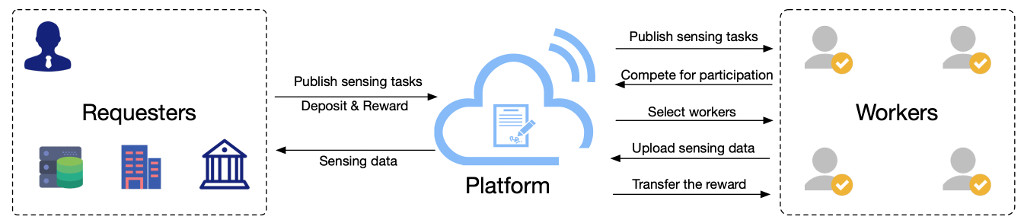
\includegraphics[width=.8\textwidth]{201909-wei-figure1.jpg}
%      \end{figure}
%\end{frame}
%
%\begin{frame}{Crowdsensing: issues}
%  		\begin{enumerate}
%   			\item Managed and maintained \alert{centralized platforms} suffer from the single point of failure
%   				\begin{itemize}
%   					\item \textbf{Proposal: } decentralized architecture (blockchain technology) that lacks a single point of failure, and enhances privacy with asymmetric encryption and digital signature technology
%   				\end{itemize}
%    		\item Encouraging workers by offering appropiate \alert{incentive mechanisms} (monetary usually) \rightarrow  \underline{auction theory} guarantees benefits for both requesters and workers\cite{paper15} but only provide short-term incentives
%    			\begin{itemize}
%   					\item \textbf{Proposal:} hybrid incentive mechanism, adopting \underline{mechanism design theory}, considering three factors:
%   					\begin{itemize}
%   					\item Monetary reward
%   					\item Reputation evaluation
%   					\item Data quality
%   					\end{itemize}
%   				\end{itemize}
%  		\end{enumerate}
%\end{frame}

% !TeX encoding = UTF-8
% !TeX root = ../main.tex

%% ------------------------------------------------------------------------
%% Copyright (C) 2021 SJTUG
%% 
%% SJTUBeamer Example Document by SJTUG
%% 
%% SJTUBeamer Example Document is licensed under a
%% Creative Commons Attribution-NonCommercial-ShareAlike 4.0 International License.
%% 
%% You should have received a copy of the license along with this
%% work. If not, see <http://creativecommons.org/licenses/by-nc-sa/4.0/>.
%% -----------------------------------------------------------------------

\section{学术论文排版}
\subsection{\LaTeX{} 排版入门}

\begin{frame}[fragile]
  \frametitle{引擎与格式}
  \begin{itemize}
    \item \textbf{引擎}:\TeX{} 的实现

          \begin{itemize}
            \item \pdfTeX{}:直接生成 PDF,支持 micro-typography
            \item \XeTeX{}:支持 Unicode、OpenType 与复杂文字编排(CTL)
            \item \LuaTeX{}:支持 Unicode,内联 Lua,支持 OpenType
            \item (u)p\TeX{}:日本方面推动,生成 |.dvi|,(支持 Unicode)
            \item Ap\TeX{}:底层 CJK 支持,内联 Ruby,Color Emoji
          \end{itemize}

    \item \textbf{格式}:\TeX{} 的语言扩展(命令封装)

          \begin{itemize}
            \item plain \TeX{}:Knuth 同志专用
            \item \LaTeX{}:排版科技类文章的事实标准
            \item Con\TeX t:基于 \LuaTeX{} 实现,优雅、易用(吗?)
          \end{itemize}

    \item \textbf{程序}:引擎 + dump 后的格式代码

          \begin{itemize}
            \item \alert{英文文章:\pdfLaTeX{}、\XeLaTeX{} 或 \LuaLaTeX{}}
            \item \alert{中文文章:\XeLaTeX{} 或 \LuaLaTeX{}}
          \end{itemize}
  \end{itemize}
\end{frame}

\begin{frame}[fragile]
  \frametitle{编译}
  \begin{itemize}
    \item 现代 \TeX{} 引擎均可直接生成 PDF
    \item 命令行

          \begin{itemize}
            \item |pdflatex|/|xelatex|/|lualatex| + |<文件名>[.tex]|
            \item 多次编译:每次均需要读取并处理中间文件
            \item 推荐 \pkg{latexmk}\footnote{\MiKTeX 用户需要自行安装 perl 解释器}:运行 |latexmk [<选项>] <文件名>| 即可自动完成所有工作
          \end{itemize}

    \item 编辑器

          \begin{itemize}
            \item 按钮的背后仍然是命令
            \item |PATH| 环境变量:确定可执行文件的位置
            \item VS Code + \LaTeX{} Workshop:配置 |tools| 和 |recipes|
          \end{itemize}
  \end{itemize}
\end{frame}


\begin{frame}[fragile]{文件结构}
  \lstset{language=[LaTeX]TeX}
  \begin{lstlisting}[basicstyle=\ttfamily]
\documentclass[a4paper]{ctexart}
% 文档类型,如 ctexart,[]内是选项,如 a4paper
% 这里开始是导言区
\usepackage{graphicx} % 引用宏包
\graphicspath{{fig/}} % 设置图片目录
% 导言区到此为止
\begin{document}
这里开始是正文
\end{document}
  \end{lstlisting}
\end{frame}

\begin{frame}[fragile]{\LaTeX{}“命令”}
  \framesubtitle{\emph{宏} (Macro)、或者\emph{控制序列} (control sequence)}
  \begin{itemize}
    \item 简单命令
          \begin{itemize}
            \item \verb|\命令|\hspace{2em}
                  \verb|{\songti 中国人民解放军}| ~$\Rightarrow$ {\songti 中国人民解放军}
            \item \verb|\命令[可选参数]{必选参数}|\\
                  \verb|\section[精简标题]{这个题目实在太长了放到目录里面不太好看}|\\
                  $\Rightarrow$ {\heiti 1.1 \hspace{1em} \songti 这个题目实在太长了放到目录里面不太好看}
          \end{itemize}
    \item 环境
          \begin{columns}[c]
            \begin{column}{0.45\textwidth}
              \begin{lstlisting}[basicstyle=\ttfamily]
\begin{equation*}
  a^2-b^2=(a+b)(a-b)
\end{equation*}
\end{lstlisting}
            \end{column}\hspace{1em}
            \begin{column}{0.45\textwidth}
              $ a^2-b^2=(a+b)(a-b)$
            \end{column}
          \end{columns}
  \end{itemize}
\end{frame}

\begin{frame}[fragile]{\LaTeX{} 常用命令}
  \begin{exampleblock}{简单命令}
    \centering
    \footnotesize
    \begin{tabular}{llll}
      \cmd{chapter}   & \cmd{section} & \cmd{subsection} & \cmd{paragraph}       \\
      章              & 节            & 小节             & 带题头段落            \\\hline
      \cmd{centering} & \cmd{emph}    & \cmd{verb}       & \cmd{url}             \\
      居中对齐        & 强调          & 原样输出         & 超链接                \\\hline
      \cmd{footnote}  & \cmd{item}    & \cmd{caption}    & \cmd{includegraphics} \\
      脚注            & 列表条目      & 标题             & 插入图片              \\\hline
      \cmd{label}     & \cmd{cite}    & \cmd{ref}                                \\
      标号            & 引用参考文献  & 引用图表公式等                           \\\hline
    \end{tabular}
  \end{exampleblock}
\end{frame}
\begin{frame}[fragile]{\LaTeX{} 常用环境}
  \begin{exampleblock}{环境}
    \centering
    \footnotesize
    \begin{tabular}{lll}
      \env{table}   & \env{figure}    & \env{equation}    \\
      表格          & 图片            & 公式              \\\hline
      \env{itemize} & \env{enumerate} & \env{description} \\
      无编号列表    & 编号列表        & 描述              \\\hline
    \end{tabular}
  \end{exampleblock}
\end{frame}
%
\begin{frame}{\LaTeX{}命令举例}
  \cmdxmp{chapter}{前言}{\heiti 第 1 章\hspace{1em} 前言}
  \cmdxmp{section[精简标题]}{这个题目实在太长了放到目录里面不太好看}{\heiti 1.1
    \hspace{1em} 这个题目实在太长了放到目录里面不太好看}
  \cmdxmp{footnote}{我是可爱的脚注}{前方高能\footnote{我是可爱的脚注}}
\end{frame}

\begin{frame}[fragile]{\LaTeX{} 环境举例}
  \begin{minipage}{0.4\linewidth}
    \begin{lstlisting}[basicstyle=\ttfamily\small]
\begin{itemize}
  \item 一条
  \item 次条
  \item 这一条可以分为 ...
    \begin{itemize}
      \item 子一条
    \end{itemize}
\end{itemize}
\end{lstlisting}
  \end{minipage}\hspace{1.5cm}
  \begin{minipage}{0.4\linewidth}
    \begin{itemize}
      \item 一条
      \item 次条
      \item 这一条可以分为 ...
            \begin{itemize}
              \item 子一条
            \end{itemize}
    \end{itemize}
  \end{minipage}
  \medskip

  \begin{minipage}{0.4\linewidth}
    \begin{lstlisting}
\begin{enumerate}
  \item 一条
  \item 次条
  \item 再条
\end{enumerate}
\end{lstlisting}
  \end{minipage}\hspace{1.5cm}
  \begin{minipage}{0.4\linewidth}
    \begin{enumerate}
      \item 一条
      \item 次条
      \item 再条
    \end{enumerate}
  \end{minipage}
\end{frame}
%

\begin{frame}[fragile]{\LaTeX{} 数学公式}

  \begin{columns}
    \begin{column}{.5\textwidth}
      \begin{lstlisting}[basicstyle=\ttfamily\small]
$V = \frac{4}{3}\pi r^3$

\[
  V = \frac{4}{3}\pi r^3
\]

\begin{equation}
\label{eq:vsphere}
V = \frac{4}{3}\pi r^3
\end{equation}
\end{lstlisting}
    \end{column}

    \begin{column}{.5\textwidth}
      $V = \frac{4}{3}\pi r^3$

      \[
        V = \frac{4}{3}\pi r^3
      \]

      \begin{equation}
        \label{eq:vsphere}
        V = \frac{4}{3}\pi r^3
      \end{equation}
    \end{column}
  \end{columns}

\end{frame}

\begin{frame}[fragile]{\LaTeX{} 数学公式}
  \begin{itemize}
    \item 数学公式排版是 \LaTeX{} 的绝对强项
    \item 数学排版需要进入数学模式,引用 \texttt{amsmath} 宏包
          \begin{itemize}
            \item 用单个美元符号(\verb|$|) 包围起来的内容是 {\bf 行内公式}
            \item 用两个美元符号(\verb|$$|) (不推荐)或 \verb|\[ \]| 包围起来的是 {\bf 单行公式} 或 {\bf 行间公式}
            \item 使用数学环境,例如 \texttt{equation} 环境内的公式会自动加上编号,
                  \texttt{align} 环境用于多行公式(例如方程组、多个并列条件等)
          \end{itemize}
    \item 寻找符号
          \begin{itemize}
            \item 运行 \texttt{texdoc symbols} 查看符号表
            \item S. Pakin. \emph{The Comprehensive \LaTeX{} Symbol List}
                  \link{https://ctan.org/pkg/comprehensive}
            \item 手写识别(有趣但不全):Detexify \link{http://detexify.kirelabs.org}
          \end{itemize}
    \item MathType 也可以使用和导出 \LaTeX{} 公式(不推荐)
  \end{itemize}
\end{frame}

\begin{frame}[fragile,label={frame:unicode-math}]{unicode-math:现代的数学输入方式}
  \LaTeX{} 的公式确实很强大,但是……符号有点难记?

  \pkg{unicode-math} 宏包提供了几乎所见即所得的公式输入(\SJTUThesis 默认使用):

  \begin{itemize}
    \item 可直接输入各类符号对应的 Unicode 字符(需要使用 UTF-8 编码):

          \begin{columns}[c]
            \begin{column}{0.45\textwidth}
              \begin{lstlisting}[basicstyle=\ttfamily]
\begin{equation*}
∫ Γ(x) dx = ±∞
\end{equation*}
      \end{lstlisting}
            \end{column}\hspace{1em}
            \begin{column}{0.45\textwidth}
              \begin{equation*}
                ∫ Γ(x) dx = ±∞
              \end{equation*}
            \end{column}
          \end{columns}
    \item 使用 |symbf| 等命令自动处理字母的粗体、斜体等变体,不必引入额外宏包。
  \end{itemize}

  \begin{columns}[c]
    \begin{column}{0.45\textwidth}
      \begin{lstlisting}[basicstyle=\ttfamily]
\begin{align*}
\symbf{\beta} &= \beta \symbf{I} \\
\symbf{a} &= a \symbf{I}
\end{align*}
\end{lstlisting}
    \end{column}\hspace{1em}
    \begin{column}{0.45\textwidth}
      \begin{align*}
        \symbf{\beta} & = \beta \symbf{I} \\
        \symbf{a}     & = a \symbf{I}
      \end{align*}
    \end{column}
  \end{columns}

\end{frame}

\begin{frame}[fragile]{层次与目录生成}
  \begin{columns}
    \begin{column}{.6\textwidth}

      \begin{lstlisting}[basicstyle=\ttfamily\small]
\tableofcontents % 这里是目录
\part{有监督学习}
\chapter{支持向量机}
\section{支持向量机简介}
\subsection{支持向量机的历史}
\subsubsection{支持向量机的诞生}
\paragraph{一些趣闻}
\subparagraph{第一个趣闻}
\end{lstlisting}
    \end{column}
    \begin{column}{.4\textwidth}
      第一部分\quad 有监督学习\\
      第一章\quad 支持向量机 \\
      1. 支持向量机简介 \\
      1.1 支持向量机的历史 \\
      1.1.1 支持向量机的诞生 \\
      一些趣闻  \\
      第一个趣闻
    \end{column}
  \end{columns}

\end{frame}


\begin{frame}[fragile]{列表与枚举}
  \begin{columns}
    \begin{column}{.6\textwidth}
      \begin{lstlisting}[basicstyle=\ttfamily\small]
\begin{enumerate}
\item \LaTeX{} 好处都有啥
  \begin{description}
    \item[好用] 体验好才是真的好
    \item[好看] 强迫症的福音
    \item[开源] 众人拾柴火焰高
  \end{description}
\item 还有呢?
  \begin{itemize}
    \item 好处 1
    \item 好处 2
  \end{itemize}
\end{enumerate}
\end{lstlisting}
    \end{column}
    \begin{column}{.4\textwidth}
      {\small
        \begin{enumerate}
          \item \LaTeX{} 好处都有啥
                \begin{description}
                  \item[好用] 体验好才是真的好
                  \item[好看] 治疗强迫症
                  \item[开源] 众人拾柴火焰高
                \end{description}
          \item 还有呢?
                \begin{itemize}
                  \item 好处 1
                  \item 好处 2
                \end{itemize}
        \end{enumerate}
      }
    \end{column}
  \end{columns}

\end{frame}


\begin{frame}[fragile]{交叉引用与插入插图}
  \begin{itemize}
    \item 给对象命名:图片、表格、公式等\\
          |\label{name}|
    \item 引用对象\\
          |\ref{name}|
  \end{itemize}
  \bigskip

  \begin{minipage}{0.7\linewidth}
    \begin{lstlisting}
交大校徽请参见图~\ref{fig:badge}。
\begin{figure}[htbp]
  \centering
  \includegraphics[height=.2\textheight]%
  {libicon.pdf}
  \caption{交大校徽。}
  \label{fig:badge}
\end{figure}
\end{lstlisting}
  \end{minipage}\hfill
  \begin{minipage}{0.3\linewidth}\centering
    {\songti 交大校徽请参见图~1。}\\[1em]
    
\includegraphics[height=0.2\textheight]{sjtu-badge-blue.pdf}\\
    {\footnotesize\heiti 图~1. 交大校徽。}
  \end{minipage}
\end{frame}

\begin{frame}[fragile]{交叉引用与插入表格}
  \begin{columns}
    \column{.6\textwidth}
    \begin{lstlisting}
\begin{table}[htbp]
   \caption{编号与含义}
   \label{tab:number}
   \centering
   \begin{tabular}{cl}
     \toprule
     编号 & 含义 \\
     \midrule
     1    & 第一 \\
     2    & 第二 \\
     \bottomrule
   \end{tabular}
\end{table}
公式~(\ref{eq:vsphere}) 中编号与含义
请参见表~\ref{tab:number}。
\end{lstlisting}
    \column{.4\textwidth}
    \centering
    {\small 表~1. 编号与含义}\\[2pt]
    \begin{tabular}{cl}\toprule
      编号 & 含义 \\\midrule
      1    & 第一 \\
      2    & 第二 \\\bottomrule
    \end{tabular}\\[5pt]

    \normalsize 公式~(\ref{eq:vsphere})编号与含义请参见表~1。
  \end{columns}
\end{frame}

\begin{frame}[fragile]{浮动体}
  \begin{itemize}
    \item 初学者最“捉摸不透”的特性之一 \link{https://liam.page/2017/03/11/floats-in-LaTeX-basic}
    \item 图片和表格有时会很大,在插入的位置不一定放得下,因此需要浮动调整
    \item 避免在文中使用「下图」「上图」的说法,而是使用图表的编号,例如 |图~\ref{fig:fig1}| 。
    \item |\begin{figure}[<位置>] 图片 \end{figure}|
          \begin{itemize}
            \item 位置参数指定浮动体摆放的偏好
            \item |h| 当前位置(here), |t| 顶部(top), |b| 底部(bottom), |p| 单独成页(p)
            \item |!h| 表示忽略一些限制,|H| 表示强制\alert{(强烈不建议,除非你知道自己在做什么)}
          \end{itemize}
    \item 温馨提示:图标题一般在下方,表标题一般在上方
  \end{itemize}
\end{frame}

\begin{frame}[fragile]
  \frametitle{作图与插图}
  \begin{itemize}
    \item 外部插入

          \begin{itemize}
            \item Mathematica、MATLAB
            \item PowerPoint、Visio、Adobe Illustrator、Inkscape
            \item Python \pkg{Matplotlib} 库、\texttt{Plots.jl}、R、Plotly 等
            \item draw.io \link{https://draw.io/}、ProcessOn \link{https://www.processon.com/} 等在线绘图网站
          \end{itemize}

    \item \TeX{} 内联

          \begin{itemize}
            \item Asymptote
            \item \alert{\pkg{pgf}/\pkg{TikZ}、\pkg{pgfplots}}
          \end{itemize}

    \item 插图格式

          \begin{itemize}
            \item 矢量图:|.pdf|
            \item 位图:|.jpg| 或 |.png|
            \item \alert{不再推荐 \texttt{.eps}}
            \item 不(完全)支持 |.svg|、|.bmp|
          \end{itemize}

    \item 一些参考:\link{https://www.zhihu.com/question/21664179}
          \link{https://tex.stackexchange.com/q/158668}
          \link{https://tex.stackexchange.com/q/72930}
  \end{itemize}
\end{frame}

\begin{frame}[fragile]{表格绘制}
  \begin{itemize}
    \item 使用 \pkg{booktabs}、\pkg{longtables}、\pkg{multirow} 等宏包
    \item 手动绘制表格确实比较令人头疼,且较难维护
    \item 推荐使用在线工具绘制后导出代码:\LaTeX{} Table Generator \link{https://www.tablesgenerator.com/latex_tables}
  \end{itemize}
\end{frame}

\begin{frame}[fragile]{文献引用}
  \begin{itemize}
    \item 新时期我国信息技术产业的发展 \cite{devoftech}
    \item 他改变了中国 \cite{thelegendofjiang}
  \end{itemize}
\end{frame}

\begin{frame}[fragile]
  \frametitle{宏包推荐(\textbf{先读文档}后使用)}
  \setlength{\leftmarginii}{1.5em}
  \vspace{-1.5em}
  \begin{multicols}{3}
    \begin{itemize}
      \item 必备

            \begin{itemize}
              \item \pkg{amsmath}
              \item \pkg{graphicx}
              \item \pkg{hyperref}
            \end{itemize}

      \item 样式

            \begin{itemize}
              \item \pkg{caption}
              \item \pkg{enumitem}
              \item \pkg{fancyhdr}
              \item \pkg{footmisc}
              \item \pkg{geometry}
              \item \pkg{titlesec}
            \end{itemize}

      \item 数学

            \begin{itemize}
              \item \pkg{bm}
              \item \pkg{mathtools}
              \item \pkg{physics}
              \item \pkg{unicode-math}
            \end{itemize}

      \item 表格

            \begin{itemize}
              \item \pkg{array}
              \item \pkg{booktabs}
              \item \pkg{longtable}
              \item \pkg{tabularx}
            \end{itemize}

      \item 插图、绘图

            \begin{itemize}
              \item \pkg{float}
              \item \pkg{pdfpages}
              \item \pkg{standalone}
              \item \pkg{subfig}
              \item \pkg{pgf}/\pkg{tikz}
              \item \pkg{pgfplots}
            \end{itemize}

      \item 字体

            \begin{itemize}
              \item \pkg{newpx}
              \item \pkg{pifont}
              \item \pkg{fontspec}
            \end{itemize}

      \item 各种功能

            \begin{itemize}
              \item \pkg{algorithm2e}
              \item \pkg{beamer}
              \item \pkg{biblatex}
              \item \pkg{listings}
              \item \pkg{mhchem}
              \item \pkg{microtype}
              \item \pkg{minted}
              \item \pkg{natbib}
              \item \pkg{siunitx}
              \item \pkg{xcolor}
            \end{itemize}

      \item 多语言

            \begin{itemize}
              \item \pkg{babel}
              \item \pkg{polyglossia}
              \item \pkg{ctex}
              \item \pkg{xeCJK}
            \end{itemize}
    \end{itemize}
  \end{multicols}
  \vspace*{-0.5cm}
\end{frame}

\subsection{论文模板使用}

\begin{frame}{模板是什么?}
  \begin{itemize}
    \item 模板
          \begin{itemize}
            \item 已经设计好的格式框架
            \item 好的模板:使用户专注于内容
            \item 不应将时间花费在调整框架上
          \end{itemize}
    \item 再提 Office 和 Word
          \begin{itemize}
            \item 很少有人会有意识地在 Word 中使用模板
            \item 定义自己的标题?定义自己的列表?定义自己的段落样式?
            \item 自动化,还是手工调?
            \item 经常被折腾的精疲力竭
            \item 学习 \LaTeX{} 能帮助自己更好科学地使用 Word
          \end{itemize}
  \end{itemize}
\end{frame}

\begin{frame}{论文排版}
  \begin{itemize}
    \item 获取模板
          \begin{itemize}
            \item 随发行版自带、手动网络下载
            \item 模板文档类 \texttt{.cls} 文件
            \item 示例 \texttt{.tex} 文件
          \end{itemize}
    \item 编辑 \texttt{.tex} 文件:添加用户内容
    \item 编译:生成 PDF 文档
  \end{itemize}
\end{frame}

\begin{frame}[fragile]{论文排版举例}
  \begin{exampleblock}{IEEE 期刊论文}
    \begin{itemize}
      \item 获取模板:已随发行版自带
            \begin{itemize}
              \item 在安装目录 |<prefix>\texlive\2021\texmf-dist\doc\latex\IEEEtran|
                    下找到 |bare_jrnl.tex|
              \item 复制到某个文件夹(比如个人存论文的目录)
            \end{itemize}
      \item 编辑 |bare_jrnl.tex| 文件 (英文模板:不支持中文)
      \item 编译
            \begin{itemize}
              \item 英文文献:\XeLaTeX{}、\pdfLaTeX{} 编译均可
            \end{itemize}
    \end{itemize}
  \end{exampleblock}
\end{frame}
% !TeX encoding = UTF-8
% !TeX root = ../main.tex

%% ------------------------------------------------------------------------
%% Copyright (C) 2021 SJTUG
%% 
%% SJTUBeamer Example Document by SJTUG
%% 
%% SJTUBeamer Example Document is licensed under a
%% Creative Commons Attribution-NonCommercial-ShareAlike 4.0 International License.
%% 
%% You should have received a copy of the license along with this
%% work. If not, see <http://creativecommons.org/licenses/by-nc-sa/4.0/>.
%% -----------------------------------------------------------------------

\section{学位论文排版}
\subsection{\SJTUThesis 上海交通大学学位论文模板}

\begin{frame}{\SJTUThesis}
  \framesubtitle{上海交通大学学位论文 \LaTeX{} 模板}
  \begin{itemize}
    \item 最早由韦建文于 2009 年 11 月发布 0.1a 版,2018 年起由 SJTUG 接手维护
    \item 最新版:\SJTUThesisVersion{} (\SJTUThesisDate)
    \item 支持本科、硕士、博士学位论文以及课程论文的排版
  \end{itemize}
  \begin{figure}[htbp]
    \centering
    
\includegraphics[height=.4\textheight]{sjtuthesis-bachelor-crop.pdf}\hspace{6pt}
    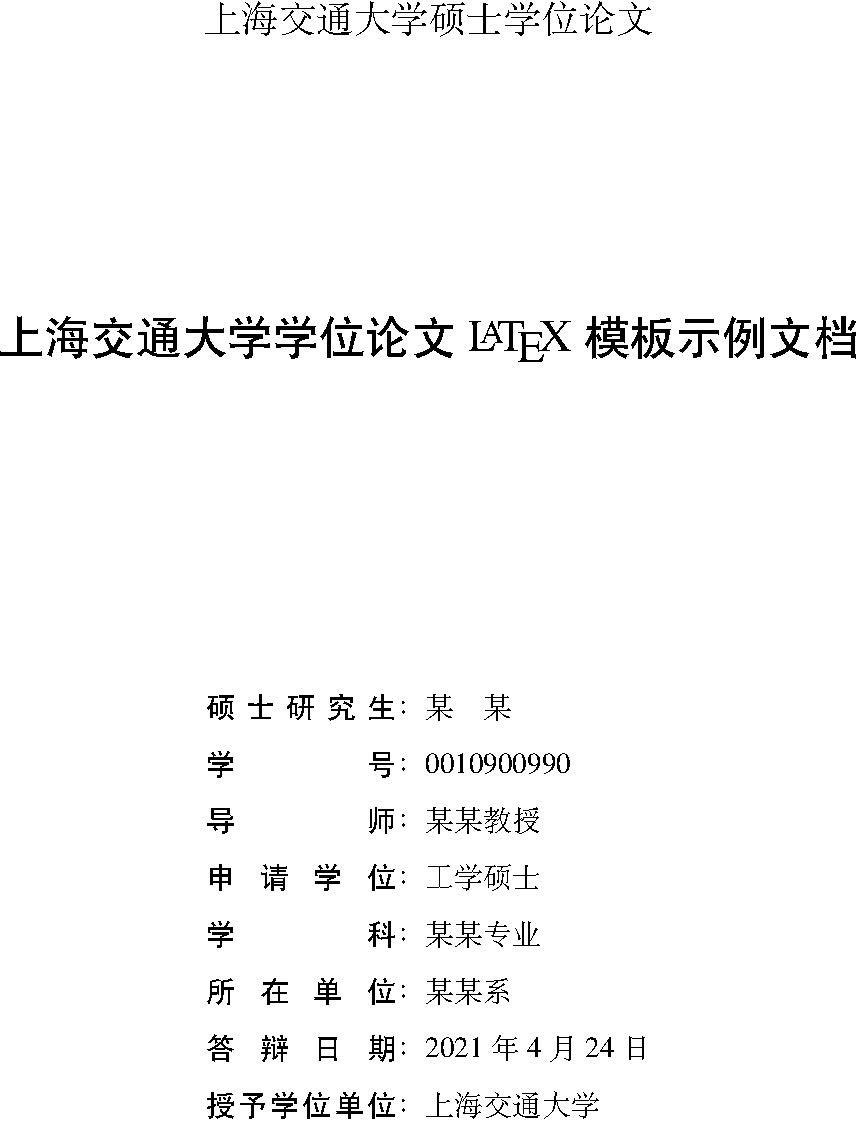
\includegraphics[height=.4\textheight]{sjtuthesis-master-crop.pdf}\hspace{6pt}
    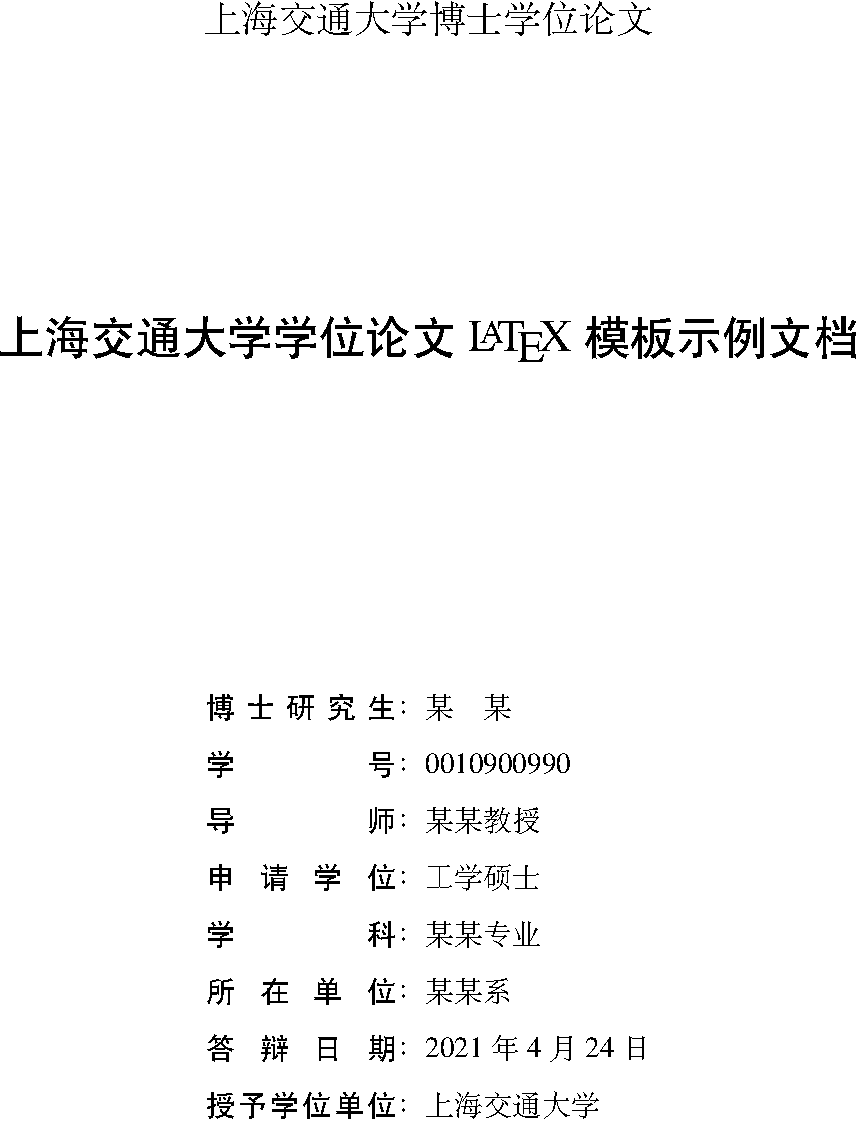
\includegraphics[height=.4\textheight]{sjtuthesis-doctor-crop.pdf}\hspace{6pt}
    
\includegraphics[height=.4\textheight]{sjtuthesis-course-crop.pdf}
  \end{figure}
\end{frame}

\begin{frame}[fragile]{获取\SJTUThesis{}}
  \begin{columns}
    \begin{column}{.65\textwidth}
      \begin{itemize}
        \item 下载最新版(推荐)
              \begin{itemize}
                \item GitHub Releases \link{https://github.com/sjtug/SJTUThesis/releases}
                \item OverLeaf \link{https://www.overleaf.com/latex/templates/sjtuthesis-latex-thesis-template-for-shanghai-jiao-tong-university/mkdwbyjbtfgg?r=b3b31f49&rm=d&rs=b}
              \end{itemize}
        \item 下载最新开发版(高级 / 想尝鲜 / 着急的用户)
              \begin{itemize}
                \item \url{https://github.com/sjtug/SJTUThesis}
                \item 切换到 |develop| 分支,点右边栏
                      \href{https://github.com/sjtug/SJTUThesis/archive/dev.zip}%
                      {Download ZIP} 按钮
              \end{itemize}
        \item 编译
              \begin{itemize}
                \item 解压缩看文档 |README.md|
                \item Windows: 双击 |Compile.bat| 脚本编译
                \item Linux \& macOS: 使用 |Makefile|
                \item 使用 |latexmk -xelatex main|
              \end{itemize}
      \end{itemize}
    \end{column}
    \begin{column}{.25\textwidth}
      \begin{figure}[htbp]
        \centering
        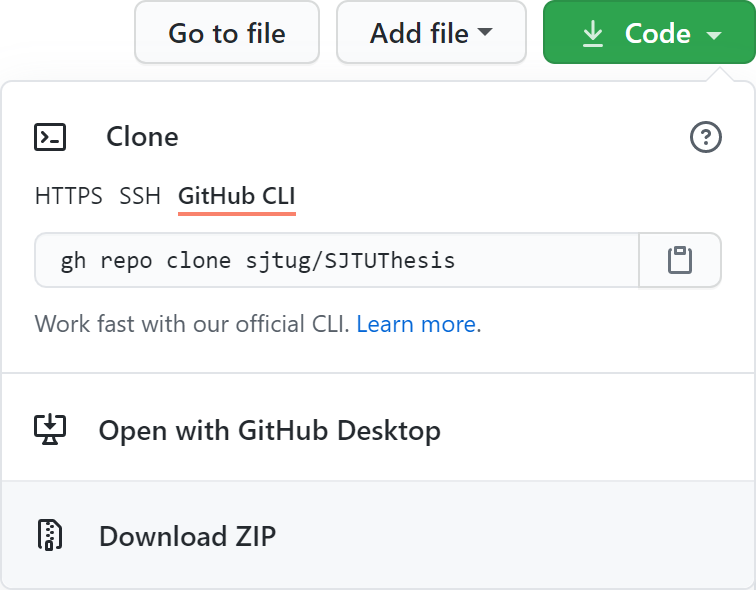
\includegraphics[width=\textwidth]{sjtuthesis-download.png}
      \end{figure}
      \vfill
    \end{column}
  \end{columns}
\end{frame}

\begin{frame}[fragile]{模板选项}
  \begin{description}
    \item[type] 指定论文类型(本科/硕士/博士/课程)
      \begin{lstlisting}[basicstyle=\ttfamily]
\documentclass[type=bachelor]{sjtuthesis}
  \end{lstlisting}
    \item[review] 开启盲审模式
      \begin{lstlisting}[basicstyle=\ttfamily]
\documentclass[type=master,review]{sjtuthesis}
  \end{lstlisting}
    \item[fontset] 指定字体(推荐使用 |windows|)
      \begin{lstlisting}[basicstyle=\ttfamily]
\documentclass[type=doctor,fontset=windows]{sjtuthesis}
  \end{lstlisting}
  \end{description}
\end{frame}

\begin{frame}[fragile]{模板设置}
  使用 |\sjtusetup| 命令指定论文各类设置:
  \begin{lstlisting}
\sjtusetup{
  info = {
    title             = {上海交通大学学位论文 \LaTeX{} 模板示例文档},
    title*            = {A Sample for \LaTeX-based SJTU Thesis Template},
    author            = {某\quad{}某},
    author*           = {Mo Mo},
  },
  style = {
    header-logo-color = red,
  },
  name = {
    publications      = {攻读学位期间完成的论文},
  },
}
  \end{lstlisting}
\end{frame}

\begin{frame}[fragile]{信息录入}
  |info| 域完成论文基本信息录入
  \begin{table}[h]
    \centering
    \footnotesize
    \begin{tabular}{lll} \toprule
      命令作用     & 中文对应选项                      & 英文对应选项      \\ \midrule
      论文标题     & |title|                           & |title*|          \\
      关键字列表   & |keywords|                        & |keywords*|       \\
      作者姓名     & |author|                          & |author*|         \\
      申请学位名称 & |degree|                          & |degree*|         \\
      院系名称     & |department|                      & |department*|     \\
      专业名称     & |major|                           & |major*|          \\
      导师         & |supervisor|                      & |supervisor*|     \\
      副导师       & |assisupervisor|                  & |assisupervisor*| \\
      日期         & \multicolumn{2}{c}{\texttt{date}}                     \\
      学号         & \multicolumn{2}{c}{\texttt{id}}                       \\ \bottomrule
    \end{tabular}
  \end{table}
\end{frame}

\begin{frame}[fragile]{数学}
  \begin{itemize}
    \item 公式示例:\nolinkurl{contents/math_and_citations.tex}
    \item \SJTUThesis{} 定义了常用的数学环境(需要手工引入 |amsthm| 宏包):
          \begin{table}[h]
            \centering
            \footnotesize
            \begin{tabular}{*{7}{l}}\toprule
              assumption & axiom   & conjecture & corollary   & definition & example  & exercise \\
              假设       & 公理    & 猜想       & 推论        & 定义       & 例       & 练习     \\\midrule
              lemma      & problem & proof      & proposition & remark     & solution & theorem  \\
              引理       & 问题    & 证明       & 命题        & 注         & 解       & 定理     \\\bottomrule
            \end{tabular}
          \end{table}
    \item \SJTUThesis{} 使用 \pkg{unicode-math} 进行数学输入(\ref{frame:unicode-math} 页),注意与传统方式的区别
  \end{itemize}
\end{frame}

\begin{frame}[fragile]{参考文献}
  \begin{itemize}
    \item 建议自动生成
          \begin{itemize}
            \item \LaTeX 引擎自身不能处理参考文献,需要借助外部程序!
          \end{itemize}
    \item 传统方法:\BibTeX 后端
          \begin{itemize}
            \item 控制文献、引用样式:\pkg{natbib} 宏包
            \item 国标样式:\pkg{gbt7714} 宏包 \link{https://mirrors.sjtug.sjtu.edu.cn/ctan/biblio/bibtex/contrib/gbt7714/gbt7714.pdf}
          \end{itemize}
    \item 现代方法:|biber| 后端 + \pkg{biblatex} 宏包
          \begin{itemize}
            \item 国标样式:\pkg{biblatex-gbt7714-2015} 宏包 \link{https://mirrors.sjtug.sjtu.edu.cn/ctan/macros/latex/contrib/biblatex-contrib/biblatex-gb7714-2015/biblatex-gb7714-2015.pdf}
          \end{itemize}
    \item 需要多轮编译——再次推荐 latexmk
  \end{itemize}
\end{frame}

\begin{frame}[fragile]{参考文献(续)}
  \begin{itemize}
    \item 生成 |.bib| 数据库
          \begin{itemize}
            \item Google Scholar 可直接复制或者批量导出
            \item 用 Zotero、Jabref 等文献管理软件生成
          \end{itemize}
    \item 两种引用模式:
          \begin{itemize}
            \item 上标模式:如“在许多文献\textsuperscript{[12-13]}中……”
                  \begin{lstlisting}[basicstyle=\ttfamily]
    \cite{key12, key13}
          \end{lstlisting}
            \item 正文模式:如“文献~[14] 证明了……”
                  \begin{lstlisting}[basicstyle=\ttfamily]
    \parencite{key14}
          \end{lstlisting}
          \end{itemize}
  \end{itemize}
\end{frame}

\begin{frame}[fragile]{\SJTUThesis 问题}
  \begin{itemize}
    \item 常见问题
          \begin{itemize}
            \item 参考文献列表出错、缺少字体、无法编译、格式不对……
            \item 阅读模板文档 |sjtuthesis.pdf| 和 SJTUThesis 示例文档代码
            \item 查看 FAQ \link{https://github.com/sjtug/SJTUThesis/wiki/常见问题}
          \end{itemize}
    \item 主动提问
          \begin{itemize}
            \item GitHub Issues 提问:\link{https://github.com/sjtug/SJTUThesis/issues}
          \end{itemize}
  \end{itemize}
\end{frame}

% !TeX encoding = UTF-8
% !TeX root = ../main.tex

%% ------------------------------------------------------------------------
%% Copyright (C) 2021 SJTUG
%% 
%% SJTUBeamer Example Document by SJTUG
%% 
%% SJTUBeamer Example Document is licensed under a
%% Creative Commons Attribution-NonCommercial-ShareAlike 4.0 International License.
%% 
%% You should have received a copy of the license along with this
%% work. If not, see <http://creativecommons.org/licenses/by-nc-sa/4.0/>.
%% -----------------------------------------------------------------------

\section{总结}

\begin{frame}{常见 \LaTeX{} 困惑}
  \begin{itemize}
    \item \alert{编译不通过} 缺少必要宏包,命令拼写错误,括号未配对等
    \item \alert{表格图片乱跑} 非问题,\LaTeX{} 浮动定位算法 \link{https://liam.page/2017/04/30/floats-in-LaTeX-the-positioning-algorithm/}
    \item \alert{段落间距变大} 非问题,\LaTeX{} 排版算法
    \item \alert{参考文献} 推荐使用 \BibTeX{} 或者 Bib\LaTeX{}(视模板而定),也可以手写 \cmd{bibitem} \link{https://github.com/hushidong/biblatex-gb7714-2015}
  \end{itemize}
\end{frame}

\begin{frame}{系统学习}
  \begin{itemize}
    \item 包太雷 《\LaTeX{} Notes(第二版)》~(3小时)(lnotes2) \link{http://dralpha.altervista.org/zh/tech/lnotes2.pdf}
    \item Stefan Kottwitz 《LaTeX Cookbook》
    \item WikiBooks:英文 \link{https://en.wikibooks.org/wiki/LaTeX}、中文 \link{https://zh.wikibooks.org/wiki/LaTeX}
    \item 在线教程:OverLeaf 帮助文档 \link{https://www.overleaf.com/learn}
    \item 经典文档(亦可能比较过时)
          \begin{itemize}
            \item 仔细阅读《一份不太简短的~\LaTeXe{} 介绍》(lshort-zh-cn)~(1--2 天)
                  \link{https://mirrors.sjtug.sjtu.edu.cn/CTAN/info/lshort/chinese/lshort-zh-cn.pdf}
            \item 粗略阅读《\LaTeXe{} 插图指南》~(2--3 小时)
          \end{itemize}
    \item 从~\SJTUThesis{} 示例文档入手
  \end{itemize}
\end{frame}

\begin{frame}{扩展阅读}
  \begin{itemize}
    \item 一份其实很短的 \LaTeX 入门文档 (Liam Huang) \link{https://liam.page/2014/09/08/latex-introduction/}
    \item 网站推荐:
          \begin{itemize}
            \item http://www.latexstudio.net/
            \item http://www.chinatex.org/
          \end{itemize}
    \item 知乎 \LaTeX{} 专栏(偏技术)\link{http://zhuanlan.zhihu.com/LaTeX}
          % \item \LaTeX{}杂谈(刘海洋)
    \item 《\LaTeX{}入门》(刘海洋)
    \item 现代 LaTeX 入门讲座(曾祥东)\link{https://github.com/stone-zeng/latex-talk/releases/tag/2019-04-18}
    \item “黑科技”:在 \LaTeX{} 中书写 Markdown 进行排版 \link{https://liam.page/2020/03/30/writing-manuscript-in-Markdown-and-typesetting-with-LaTeX/}
  \end{itemize}
\end{frame}


\begin{frame}[fragile]{利用文档}
  \begin{itemize}
    \item 常用文档
          \begin{itemize}
            \item \pkg{symbols}: 符号大全
            \item \pkg{Mathmode}: 数学参考
            \item \pkg{ctex}, \pkg{xeCJK}: 中文支持
            \item \pkg{texlive-zh}: \TL 安装与使用
            \item 所用宏包文档
          \end{itemize}
    \item 工具
          \begin{itemize}
            \item |tlmgr|: \TL 管理器
            \item |texdoc|: \TeX{} 文档查看器\\
                  例如:|texdoc lshort-zh-cn|
            \item 在线文档 \TeX{}doc \link{http://texdoc.net/}
            \item TeX Studio 和 WinEdt 都支持在帮助里看文档
          \end{itemize}
  \end{itemize}
\end{frame}

\begin{frame}{一点人生的经验}
  \begin{itemize}
    \item 不要着急安装,先在 OverLeaf 上熟悉各类操作
    \item 不要过于相信网上的中文文档
          \begin{itemize}
            \item 简单鉴别方法: 排版的好看程度
          \end{itemize}
    \item 湿兄用U盘拷给你的的 \CTeX{} 套装一定是过时的,\SJTUThesis{} 八成是老版本的
    \item 如果你要处理中文
          \begin{itemize}
            \item 使用 \XeLaTeX{}, 使用 \XeLaTeX{}, 使用 \XeLaTeX{}
            \item 忘记 \pkg{CJK}, 忘记 \pkg{CJK}, 忘记 \pkg{CJK}
            \item 使用 \pkg{ctex} 宏包(2.0以上版本)(跟 \CTeX{} 套装仅仅是名字像)
          \end{itemize}
    \item 写一点,编译一次,减小排错搜索空间
  \end{itemize}
\end{frame}

\begin{frame}[fragile]
  \frametitle{Git版本管理}
  \begin{itemize}
    \item 版本管理的必要性
          \begin{itemize}
            \item 远离「初稿,第二稿……终稿,终稿(打死也不改了)」命名
            \item 方便与他人协同合作
          \end{itemize}
    \item 基本用法
          \begin{itemize}
            \item 跟踪更改:|git init|、|git add|、|git commit|
            \item 撤销与回滚:|git reset|、|git revert|
            \item 分支与高级用法:|git branch|、|git checkout|、|git rebase|
            \item 远端仓库操作:|git pull|、|git push|、|git fetch|
            \item 推荐用 VS Code 等进行可视化操作
            \item 参考链接:\link{https://git-scm.com/book/en/v2}
                  \link{https://www.liaoxuefeng.com/wiki/0013739516305929606dd18361248578c67b8067c8c017b000}
          \end{itemize}
    \item 在线 Git 服务
          \begin{itemize}
            \item GitHub \href{https://github.com}{\faGithub}
            \item 上海交通大学源代码管理平台(基于 GitLab) \link{https://git.sjtu.edu.cn}
          \end{itemize}
  \end{itemize}
\end{frame}

% 寻求帮助
\begin{frame}{求助}
  \begin{columns}[c]
    \begin{column}{.45\textwidth}
      \begin{itemize}
        \item BBS
              \begin{itemize}
                \item 水源社区 \link{https://dev.bbs.sjtu.edu.cn/}
                \item \sout{\CTeX 社区} (已关闭) \link{http://bbs.ctex.org/}
                \item 转移到 GitHub 的 \CTeX 社区 \link{https://github.com/CTeX-org/forum}
              \end{itemize}
        \item \TeX{} FAQ \link{https://www.texfaq.org/}
        \item \TeX{} StackExchange \link{https://tex.stackexchange.com/}
        \item Google, Bing, etc.
              \begin{itemize}
                \item 使用\textbf{英语}搜索
              \end{itemize}
      \end{itemize}
    \end{column}
    \begin{column}{.45\textwidth}
      
\includegraphics[width=\textwidth]{TFZsuperellipse-crop.pdf}
    \end{column}
  \end{columns}
\end{frame}

\begin{frame}{你也可以帮助}
  \begin{itemize}
    \item 错误反馈、改进建议:GitHub Issues \link{https://github.com/sjtug/SJTUThesis/issues}
    \item 出力维护:\LaTeX{} 宏包、模板编写,bug 修复
    \item 科普、答疑
    \item \sout{来当主讲人}
  \end{itemize}
\end{frame}

\appendix

\begin{frame}
  \frametitle{参考文献}
  \printbibliography
\end{frame}

\makebottom

\end{document}
